\definecolor{zzzzzz}{rgb}{0.7,0.7,0.7}
\definecolor{zzqqzz}{rgb}{0.6,0,0.6}
\definecolor{qqqqzz}{rgb}{0,0,0.6}

\begin{subfigure}{0.4\textwidth}
    \centering
    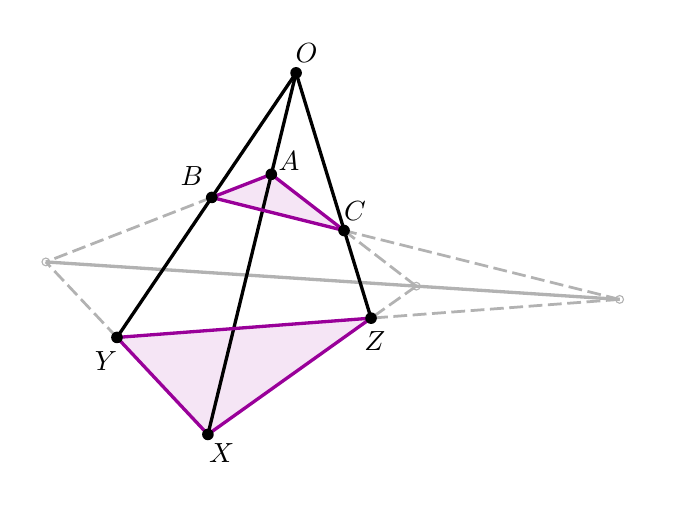
\begin{tikzpicture}[scale = 0.7]
        \clip(-4.2,-1.5) rectangle (7.04,6.74);
        \fill[line width=1.2pt,color=zzqqzz,fill=zzqqzz,fill opacity=0.1] (0.22,4.08) -- (-0.86,3.66) -- (1.54,3.06) -- cycle;
        \fill[line width=1.2pt,color=zzqqzz,fill=zzqqzz,fill opacity=0.1] (-0.93,-0.64) -- (-2.58,1.12) -- (2.03,1.47) -- cycle;
        \draw [line width=1.2pt,color=zzzzzz] (-3.87,2.49)-- (6.54,1.81);
        \draw [line width=1.2pt] (0.67,5.92)-- (-2.58,1.12);
        \draw [line width=1.2pt] (0.67,5.92)-- (2.03,1.47);
        \draw [line width=1.2pt] (0.67,5.92)-- (-0.93,-0.64);
        \draw [line width=1.2pt,color=zzqqzz] (0.22,4.08)-- (-0.86,3.66);
        \draw [line width=1.2pt,color=zzqqzz] (-0.86,3.66)-- (1.54,3.06);
        \draw [line width=1.2pt,color=zzqqzz] (1.54,3.06)-- (0.22,4.08);
        \draw [line width=1.2pt,color=zzqqzz] (-0.93,-0.64)-- (-2.58,1.12);
        \draw [line width=1.2pt,color=zzqqzz] (-2.58,1.12)-- (2.03,1.47);
        \draw [line width=1.2pt,color=zzqqzz] (2.03,1.47)-- (-0.93,-0.64);
        \draw [line width=1pt,dash pattern=on 5pt off 2pt,color=zzzzzz] (6.54,1.81)-- (1.54,3.06);
        \draw [line width=1pt,dash pattern=on 5pt off 2pt,color=zzzzzz] (6.54,1.81)-- (2.03,1.47);
        \draw [line width=1pt,dash pattern=on 5pt off 2pt,color=zzzzzz] (2.85,2.05)-- (2.03,1.47);
        \draw [line width=1pt,dash pattern=on 5pt off 2pt,color=zzzzzz] (2.85,2.05)-- (1.54,3.06);
        \draw [line width=1pt,dash pattern=on 5pt off 2pt,color=zzzzzz] (-0.86,3.66)-- (-3.87,2.49);
        \draw [line width=1pt,dash pattern=on 5pt off 2pt,color=zzzzzz] (-2.58,1.12)-- (-3.87,2.49);
        \begin{scriptsize}
            \normalsize
            \fill [color=black] (0.22,4.08) circle (3.0pt);
            \draw[color=black] (0.54,4.32) node {$A$};
            \fill [color=black] (-0.86,3.66) circle (3.0pt);
            \draw[color=black] (-1.22,4.05) node {$B$};
            \fill [color=black] (1.54,3.06) circle (3.0pt);
            \draw[color=black] (1.74,3.42) node {$C$};
            \fill [color=black] (0.67,5.92) circle (3.0pt);
            \draw[color=black] (0.86,6.28) node {$O$};
            \fill [color=black] (-0.93,-0.64) circle (3.0pt);
            \draw[color=black] (-0.68,-0.98) node {$X$};
            \fill [color=black] (-2.58,1.12) circle (3.0pt);
            \draw[color=black] (-2.78,0.7) node {$Y$};
            \fill [color=black] (2.03,1.47) circle (3.0pt);
            \draw[color=black] (2.1,1.05) node {$Z$};
            \draw [color=zzzzzz] (-3.87,2.49) circle (2.0pt);
            \draw [color=zzzzzz] (6.54,1.81) circle (2.0pt);
            \draw [color=zzzzzz] (2.85,2.05) circle (2.0pt);
            \fill [color=black] (7.19,-1.64) circle (2.0pt);
        \end{scriptsize}
    \end{tikzpicture}
    \caption{Perspectiva con respecto a un punto.}
\end{subfigure}
\hspace{0.1\textwidth}
\begin{subfigure}{0.4\textwidth}
    \centering
    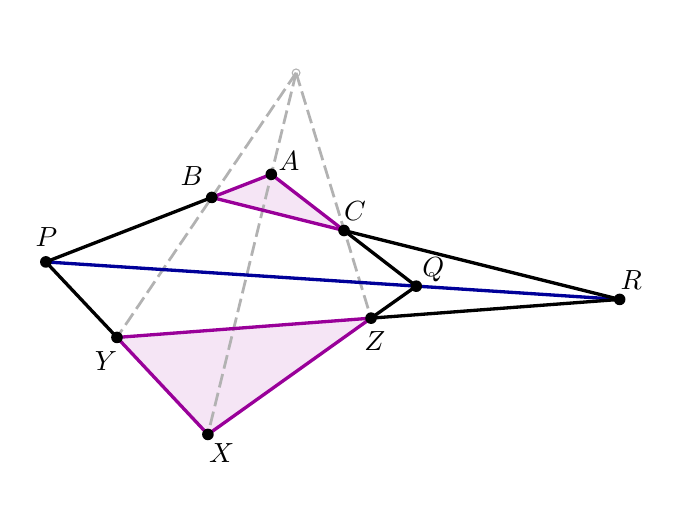
\begin{tikzpicture}[scale = 0.7]
        \clip(-4.2,-1.5) rectangle (7.04,6.74);
        \fill[line width=1.2pt,color=zzqqzz,fill=zzqqzz,fill opacity=0.1] (0.22,4.08) -- (-0.86,3.66) -- (1.54,3.06) -- cycle;
        \fill[line width=1.2pt,color=zzqqzz,fill=zzqqzz,fill opacity=0.1] (-0.93,-0.64) -- (-2.58,1.12) -- (2.03,1.47) -- cycle;
        \draw [line width=1pt,dash pattern=on 5pt off 2pt,color=zzzzzz] (0.67,5.92)-- (-2.58,1.12);
        \draw [line width=1pt,dash pattern=on 5pt off 2pt,color=zzzzzz] (0.67,5.92)-- (2.03,1.47);
        \draw [line width=1pt,dash pattern=on 5pt off 2pt,color=zzzzzz] (0.67,5.92)-- (-0.93,-0.64);
        \draw [line width=1.2pt,color=zzqqzz] (0.22,4.08)-- (-0.86,3.66);
        \draw [line width=1.2pt,color=zzqqzz] (-0.86,3.66)-- (1.54,3.06);
        \draw [line width=1.2pt,color=zzqqzz] (1.54,3.06)-- (0.22,4.08);
        \draw [line width=1.2pt,color=zzqqzz] (-0.93,-0.64)-- (-2.58,1.12);
        \draw [line width=1.2pt,color=zzqqzz] (-2.58,1.12)-- (2.03,1.47);
        \draw [line width=1.2pt,color=zzqqzz] (2.03,1.47)-- (-0.93,-0.64);
        \draw [line width=1.2pt,color=qqqqzz] (-3.87,2.49)-- (6.54,1.81);
        \draw [line width=1.2pt] (6.54,1.81)-- (1.54,3.06);
        \draw [line width=1.2pt] (6.54,1.81)-- (2.03,1.47);
        \draw [line width=1.2pt] (2.85,2.05)-- (2.03,1.47);
        \draw [line width=1.2pt] (2.85,2.05)-- (1.54,3.06);
        \draw [line width=1.2pt] (-0.86,3.66)-- (-3.87,2.49);
        \draw [line width=1.2pt] (-2.58,1.12)-- (-3.87,2.49);
        \begin{scriptsize}
            \normalsize
            \fill [color=black] (0.22,4.08) circle (3.0pt);
            \draw[color=black] (0.54,4.32) node {$A$};
            \fill [color=black] (-0.86,3.66) circle (3.0pt);
            \draw[color=black] (-1.22,4.05) node {$B$};
            \fill [color=black] (1.54,3.06) circle (3.0pt);
            \draw[color=black] (1.74,3.42) node {$C$};
            \draw [color=zzzzzz] (0.67,5.92) circle (2.0pt);
            \fill [color=black] (-0.93,-0.64) circle (3.0pt);
            \draw[color=black] (-0.68,-0.98) node {$X$};
            \fill [color=black] (-2.58,1.12) circle (3.0pt);
            \draw[color=black] (-2.78,0.7) node {$Y$};
            \fill [color=black] (2.03,1.47) circle (3.0pt);
            \draw[color=black] (2.1,1.05) node {$Z$};
            \fill [color=black] (-3.87,2.49) circle (3.0pt);
            \draw[color=black] (-3.86,2.95) node {$P$};
            \fill [color=black] (6.54,1.81) circle (3.0pt);
            \draw[color=black] (6.75,2.17) node {$R$};
            \fill [color=black] (2.85,2.05) circle (3.0pt);
            \draw[color=black] (3.16,2.35) node[fill = white, rounded corners = 5pt, inner sep=0.8pt] {$Q$};
            \fill [color=black] (7.19,-1.64) circle (3.0pt);
        \end{scriptsize}
    \end{tikzpicture}
    \caption{Perspectiva con respecto a una recta.}
\end{subfigure}